\begin{figure*}[t]
\begin{minipage}[b]{0.32\linewidth}
\centering
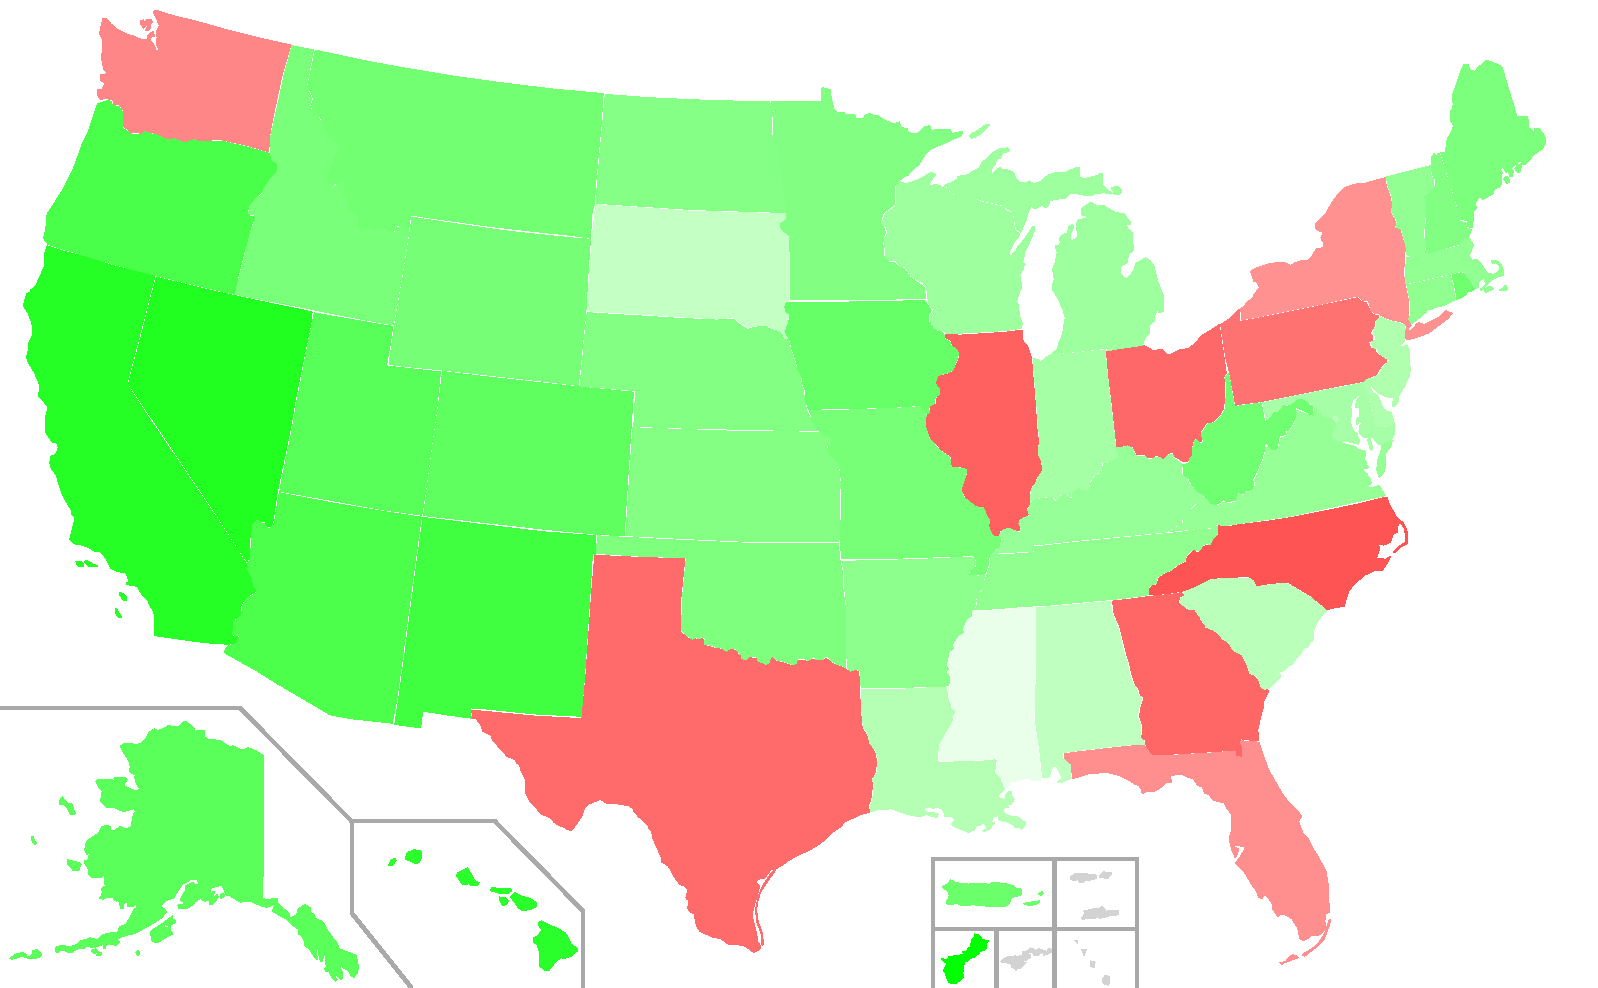
\includegraphics[width=53mm]{./images/ca.pdf}
\caption{Followers of California}
\label{fig:state-ca}
\end{minipage}
\hspace{2mm}
\begin{minipage}[b]{0.32\linewidth}
\centering
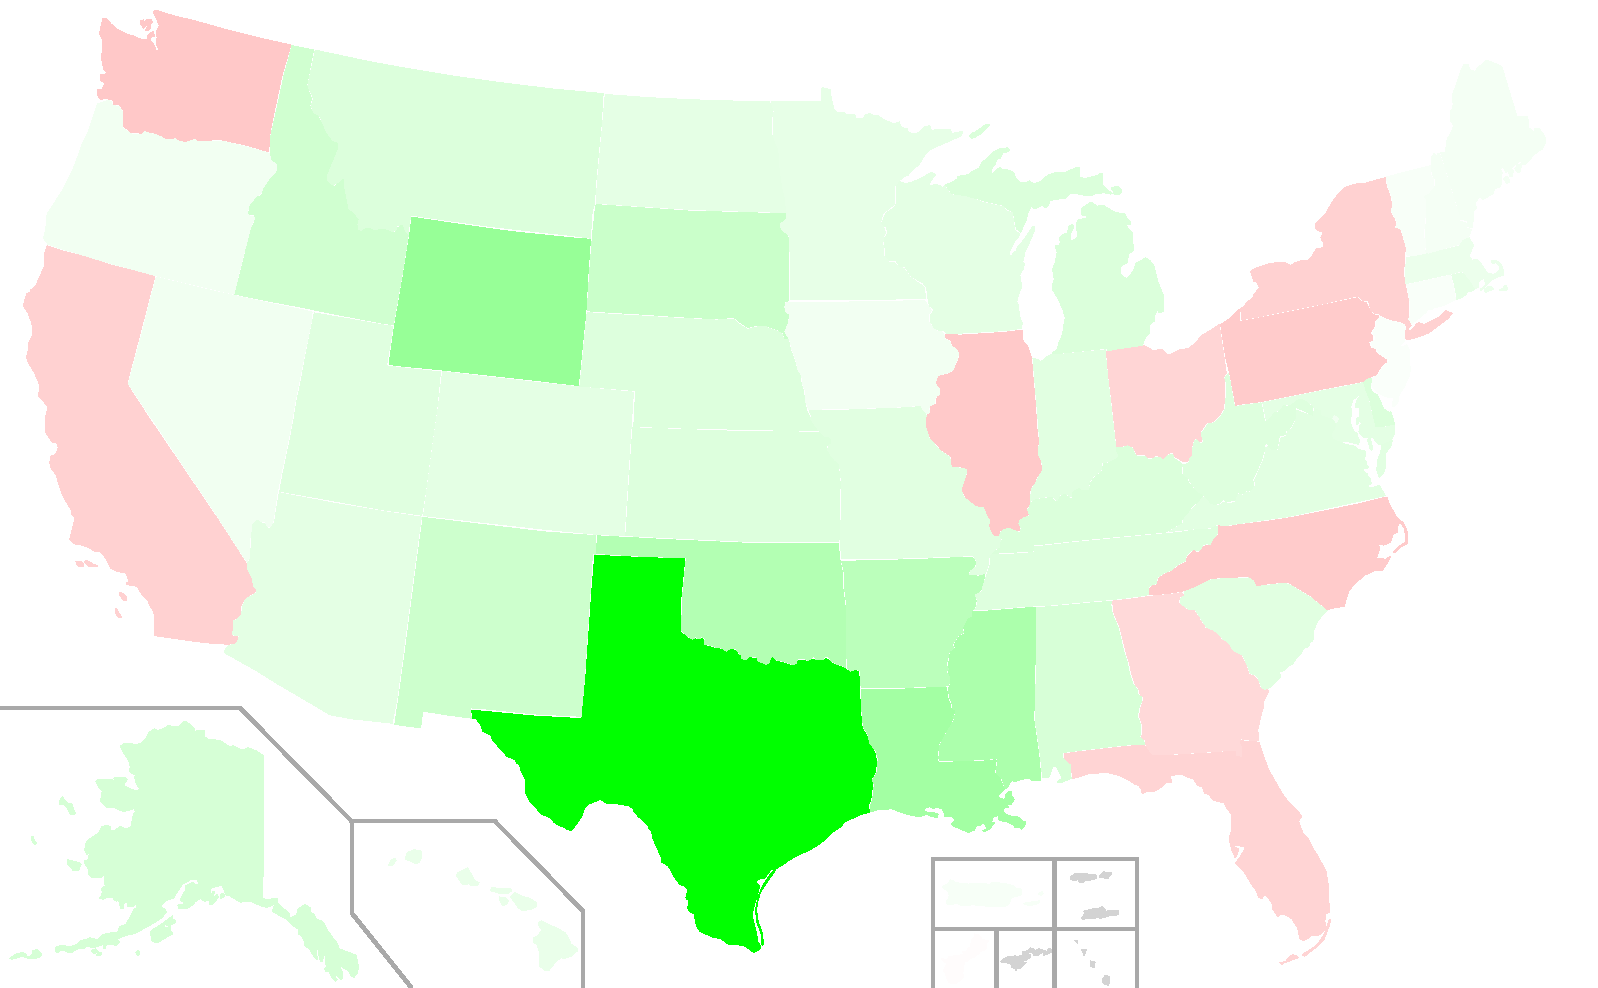
\includegraphics[width=53mm]{./images/tx.pdf}
\caption{Followers of Texas}
\label{fig:state-tx}
\end{minipage}
\hspace{2mm}
\begin{minipage}[b]{0.32\linewidth}
\centering
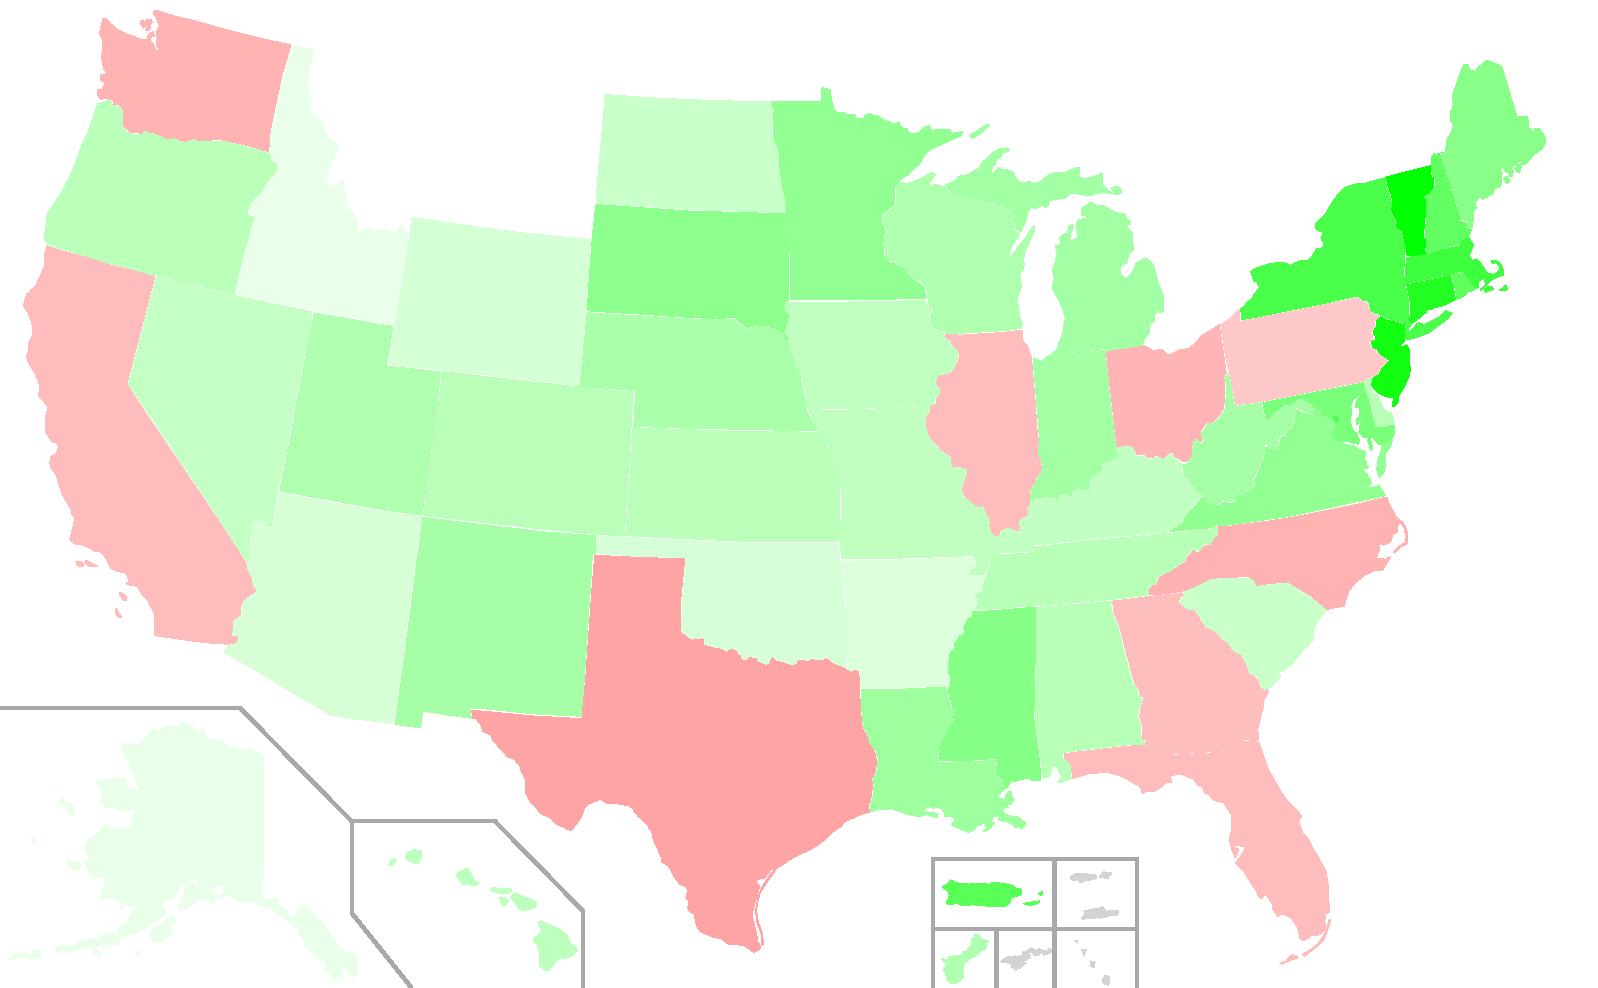
\includegraphics[width=53mm]{./images/ny.pdf}
\caption{Followers of New York}
\label{fig:state-ny}
\end{minipage}
\end{figure*}

\begin{figure*}[t]
\begin{minipage}[b]{0.32\linewidth}
\centering
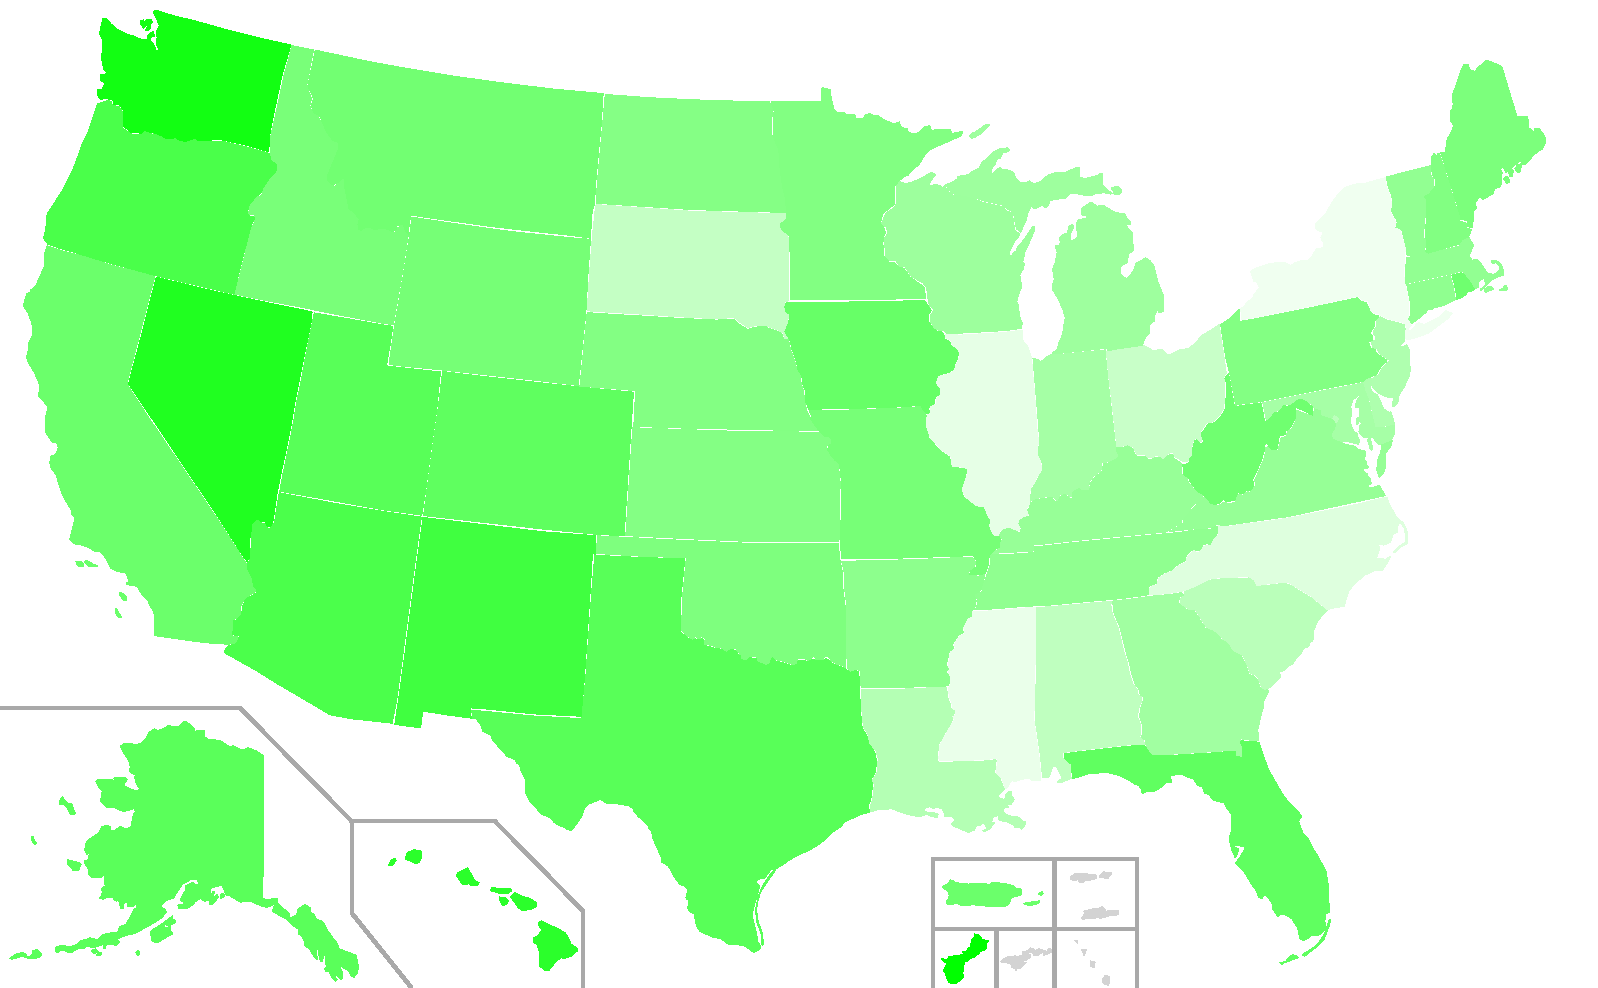
\includegraphics[width=53mm]{./images/fl.pdf}
\caption{Followers of Florida}
\label{fig:state-fl}
\end{minipage}
\hspace{2mm}
\begin{minipage}[b]{0.32\linewidth}
\centering
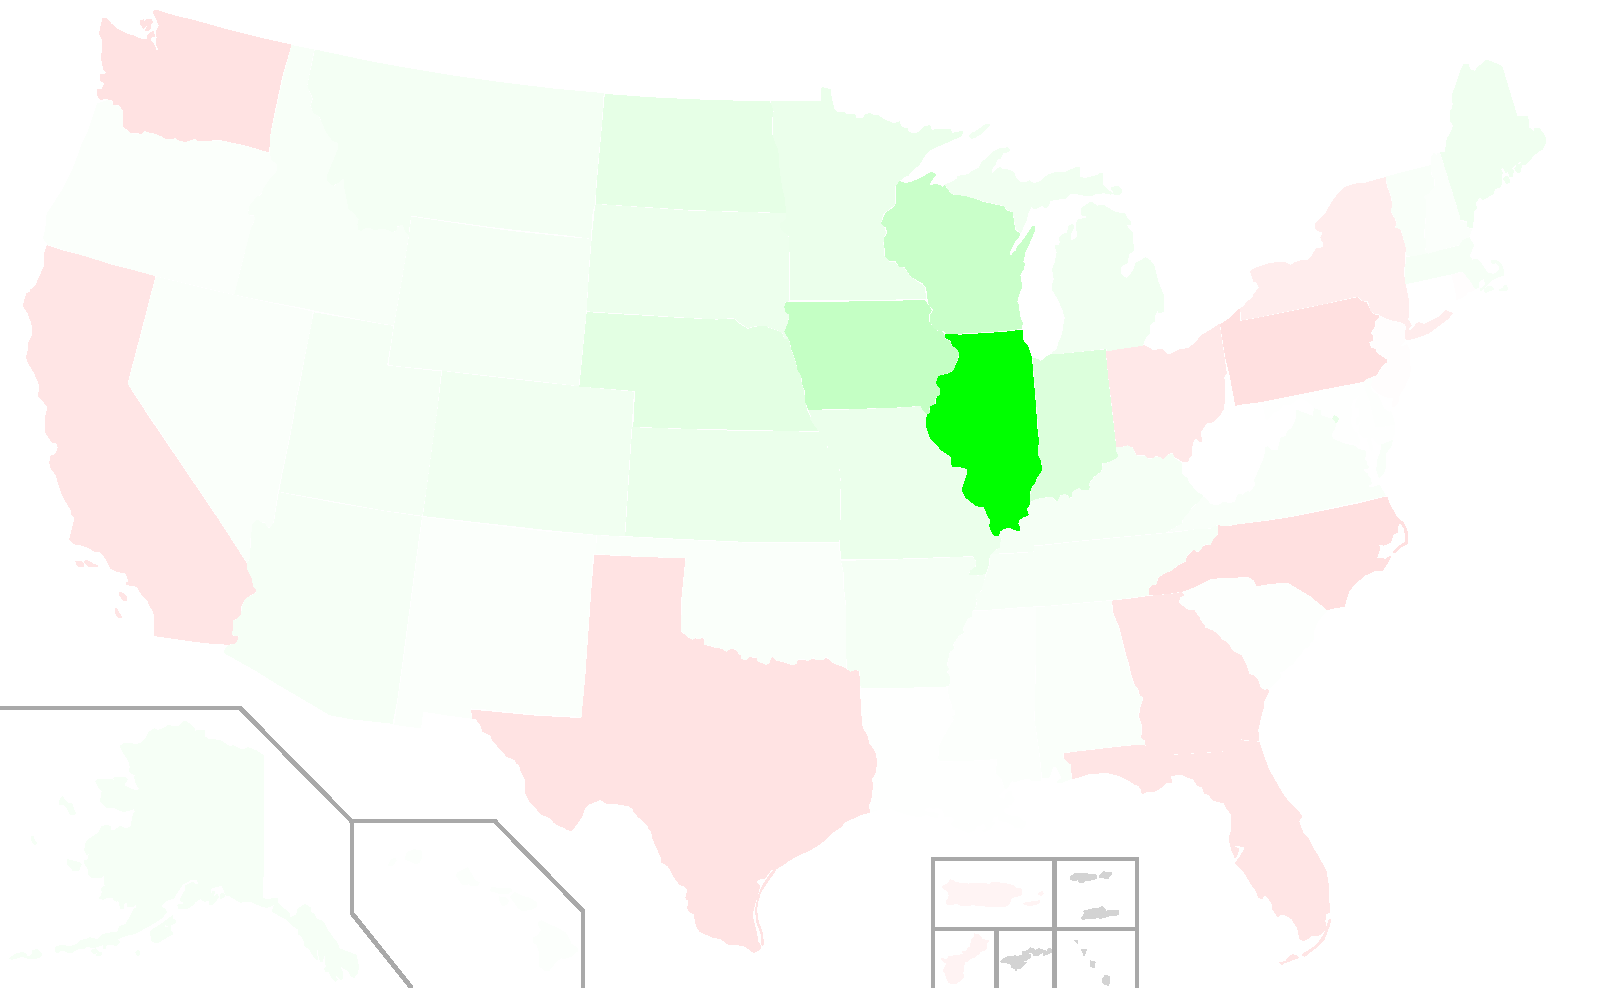
\includegraphics[width=53mm]{./images/il.pdf}
\caption{Followers of Illinois}
\label{fig:state-il}
\end{minipage}
\hspace{2mm}
\begin{minipage}[b]{0.32\linewidth}
\centering
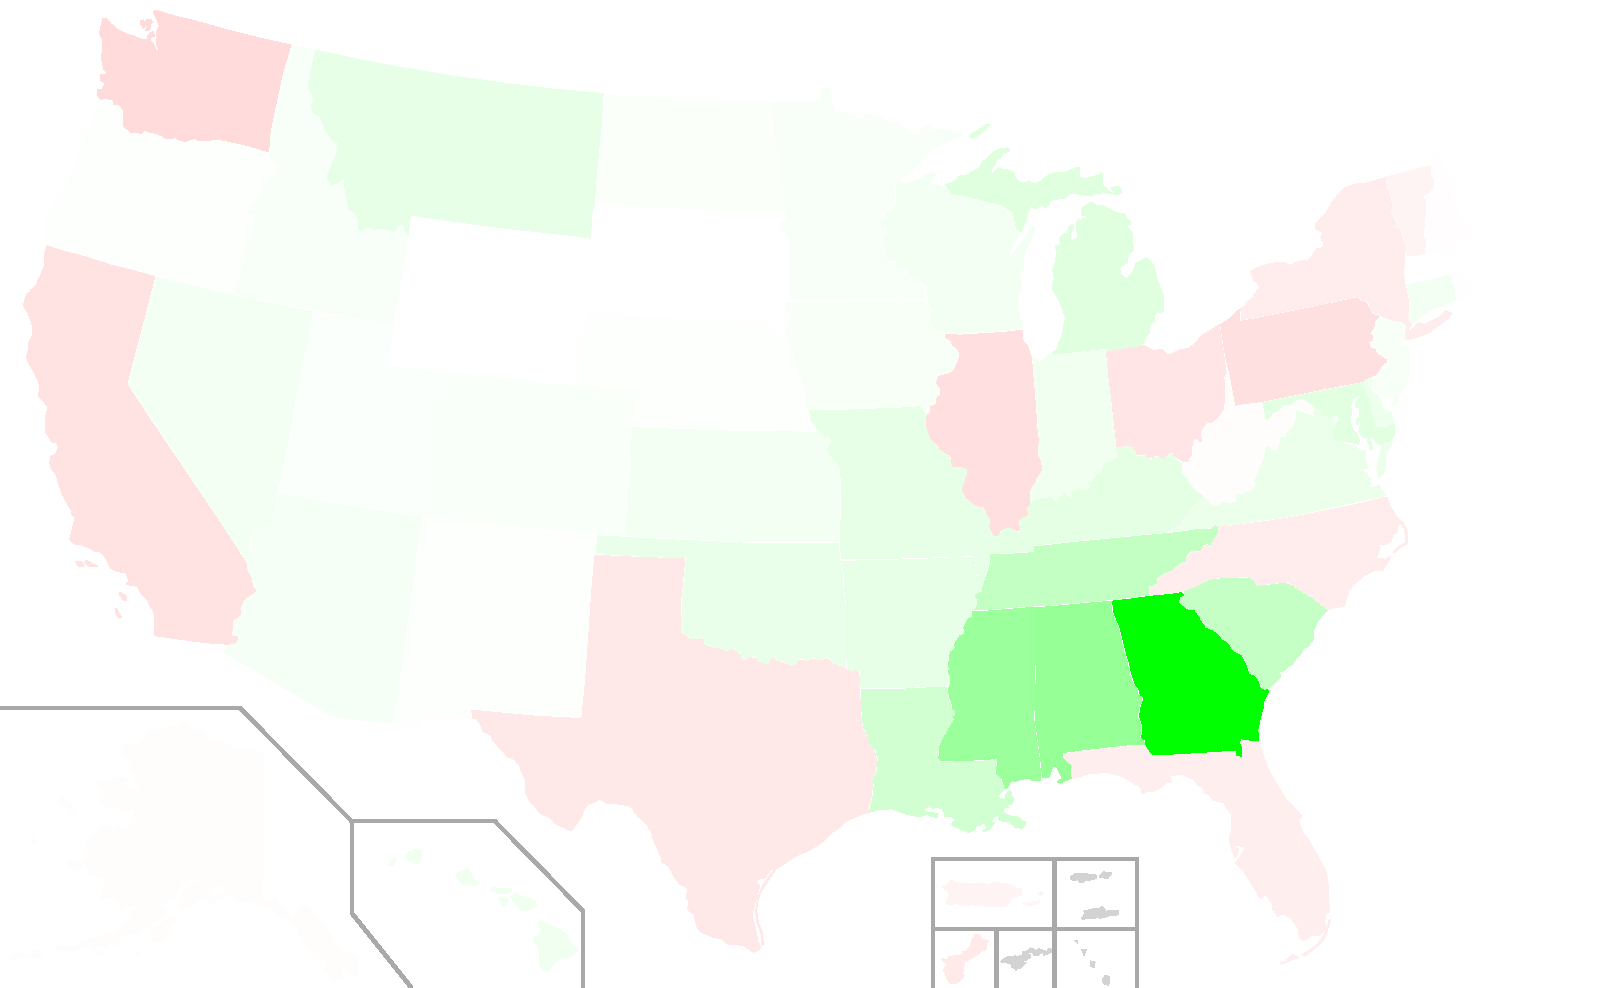
\includegraphics[width=53mm]{./images/ga.pdf}
\caption{Followers of Georgia}
\label{fig:state-ga}
\end{minipage}
\end{figure*}

\begin{figure*}[t]
\begin{minipage}[b]{0.32\linewidth}
\centering
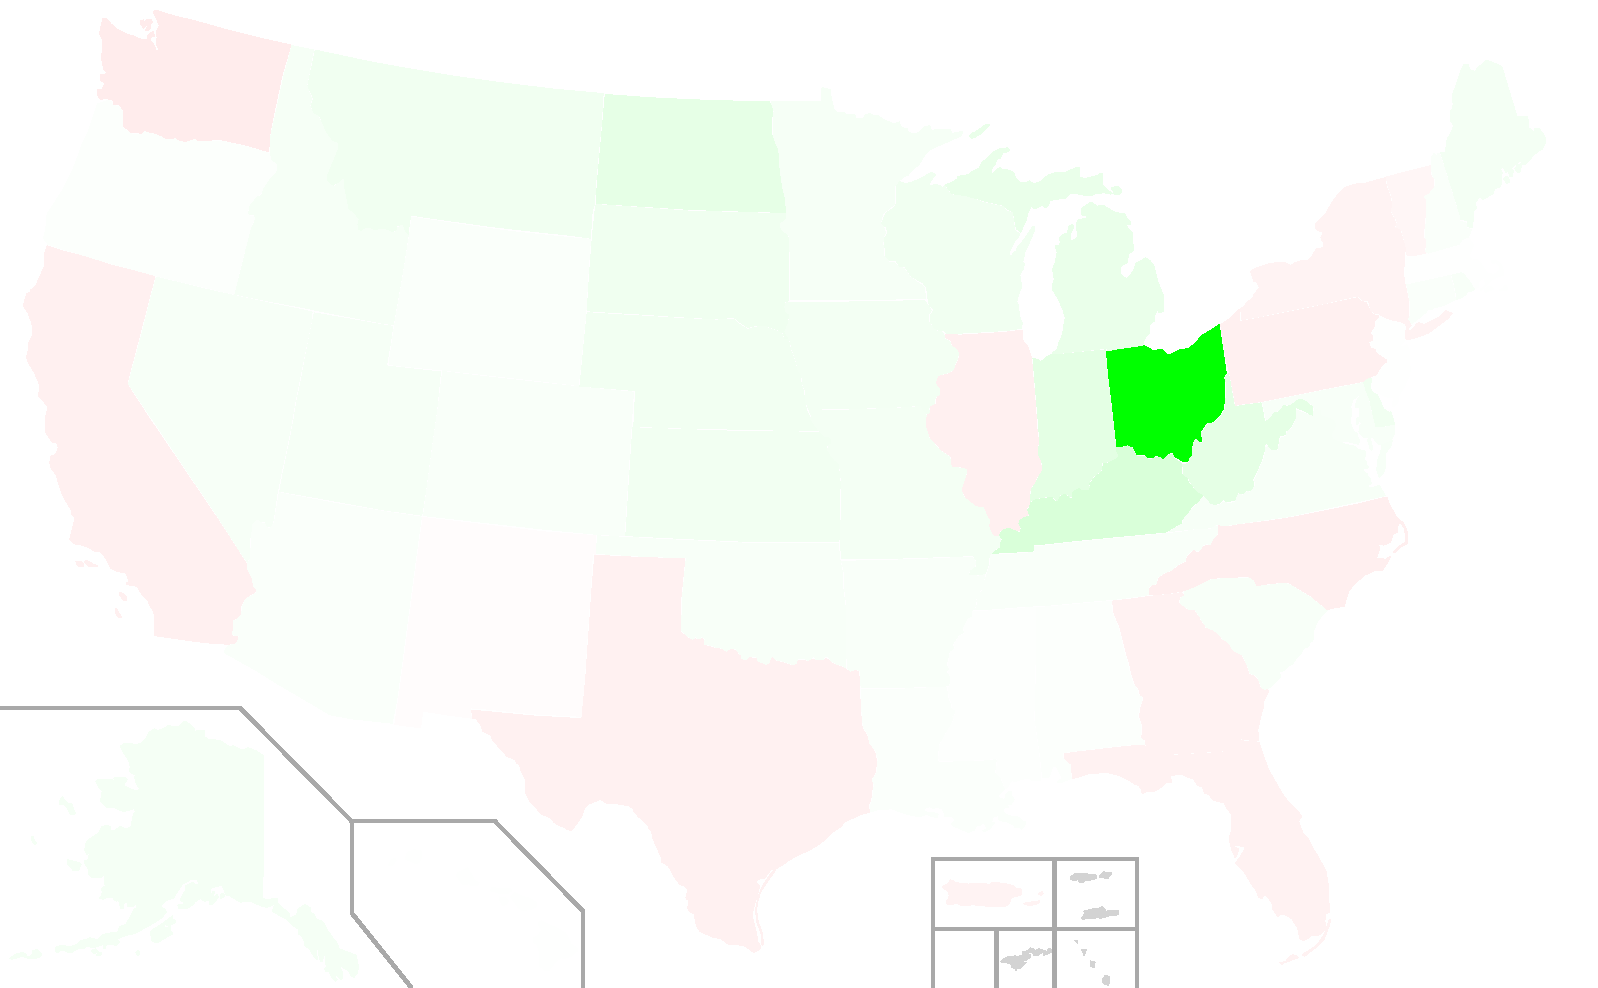
\includegraphics[width=53mm]{./images/oh.pdf}
\caption{Followers of Ohio}
\label{fig:state-oh}
\end{minipage}
\hspace{2mm}
\begin{minipage}[b]{0.32\linewidth}
\centering
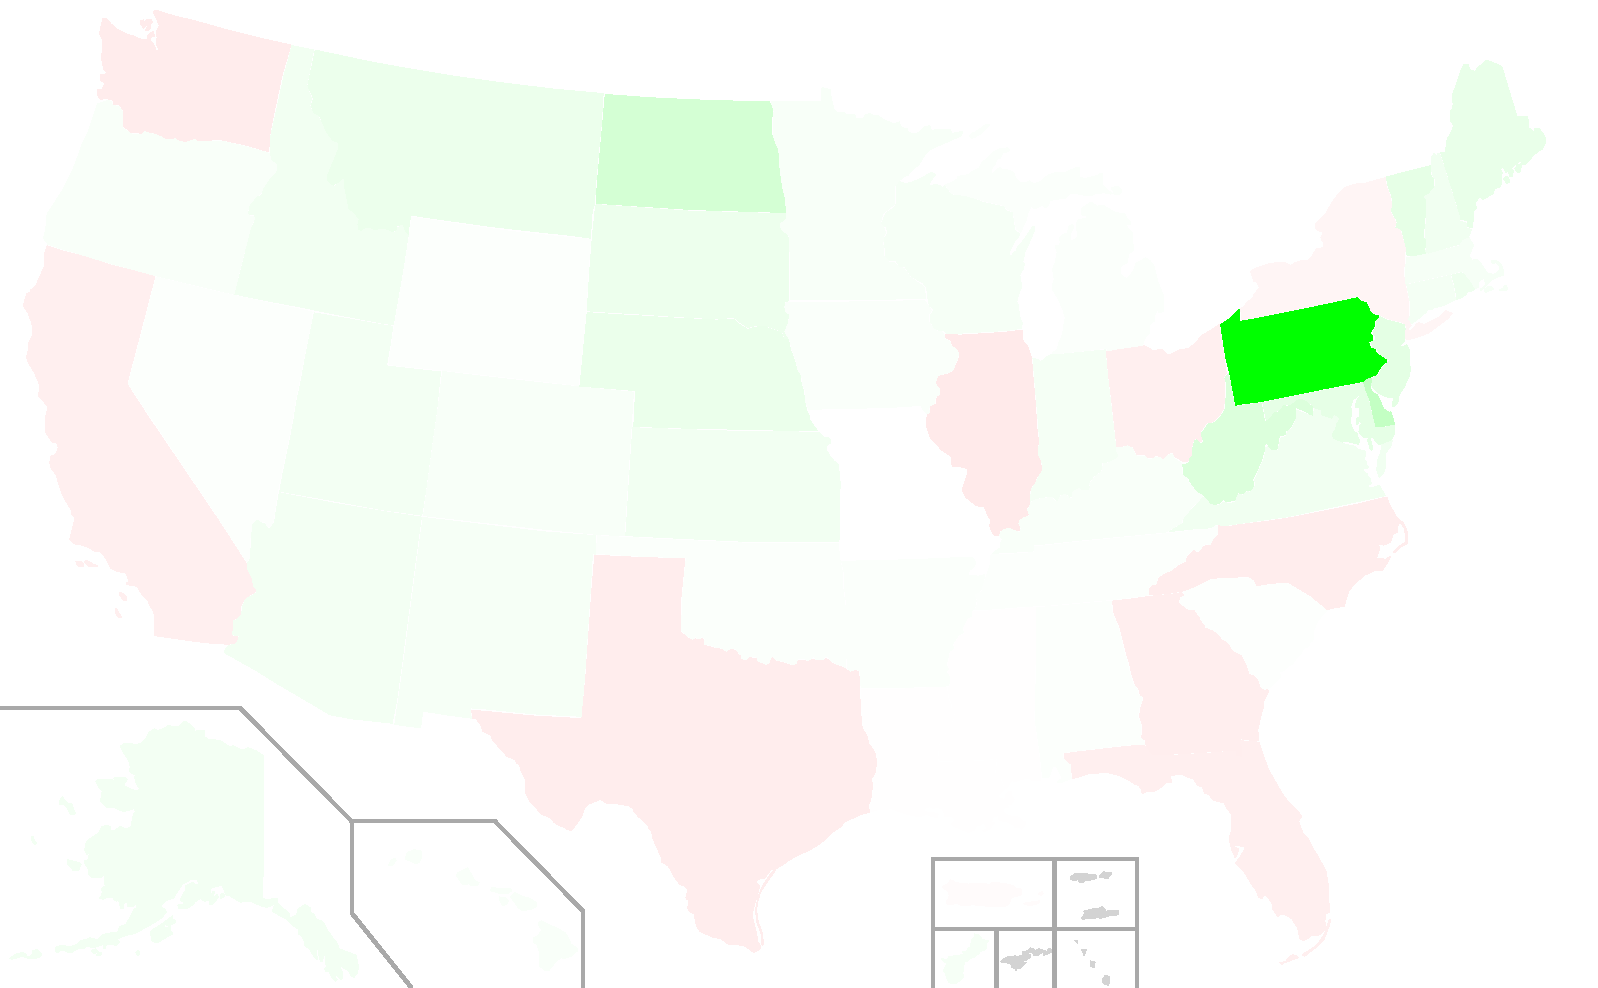
\includegraphics[width=53mm]{./images/pa.pdf}
\caption{Followers of Pennsylvania}
\label{fig:state-pa}
\end{minipage}
\hspace{2mm}
\begin{minipage}[b]{0.32\linewidth}
\centering
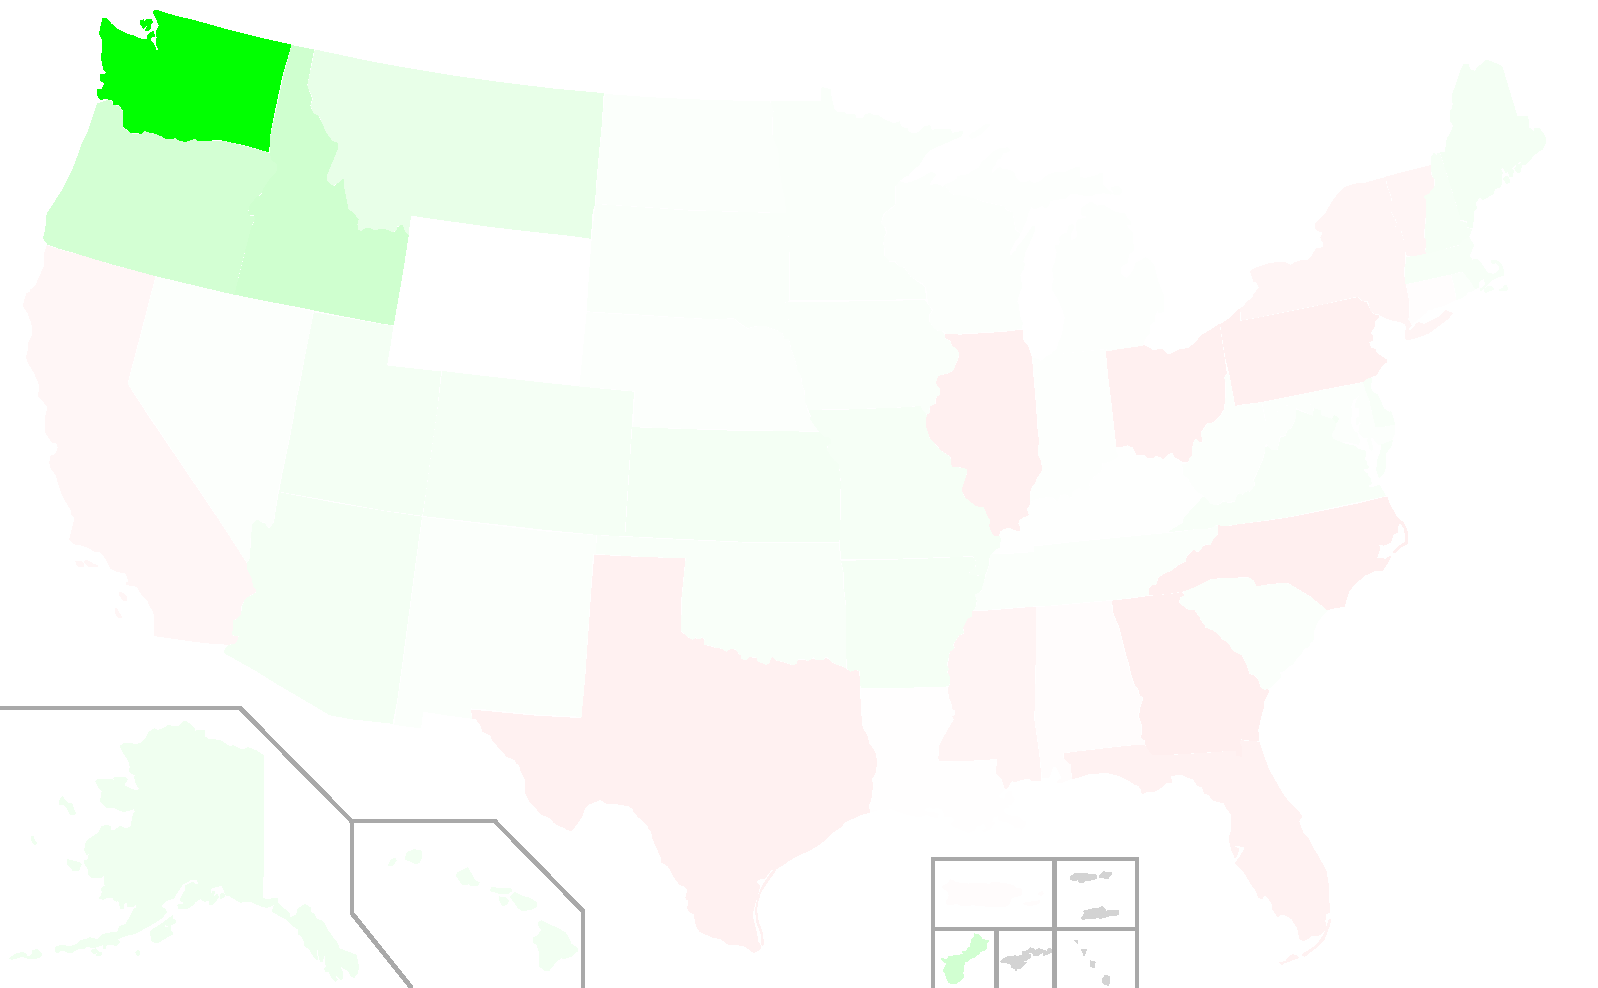
\includegraphics[width=53mm]{./images/wa.pdf}
\caption{Followers of Washington}
\label{fig:state-wa}
\end{minipage}
\end{figure*}

\begin{center}
\begin{figure*}[t]
\begin{minipage}[b]{0.32\linewidth}
\centering
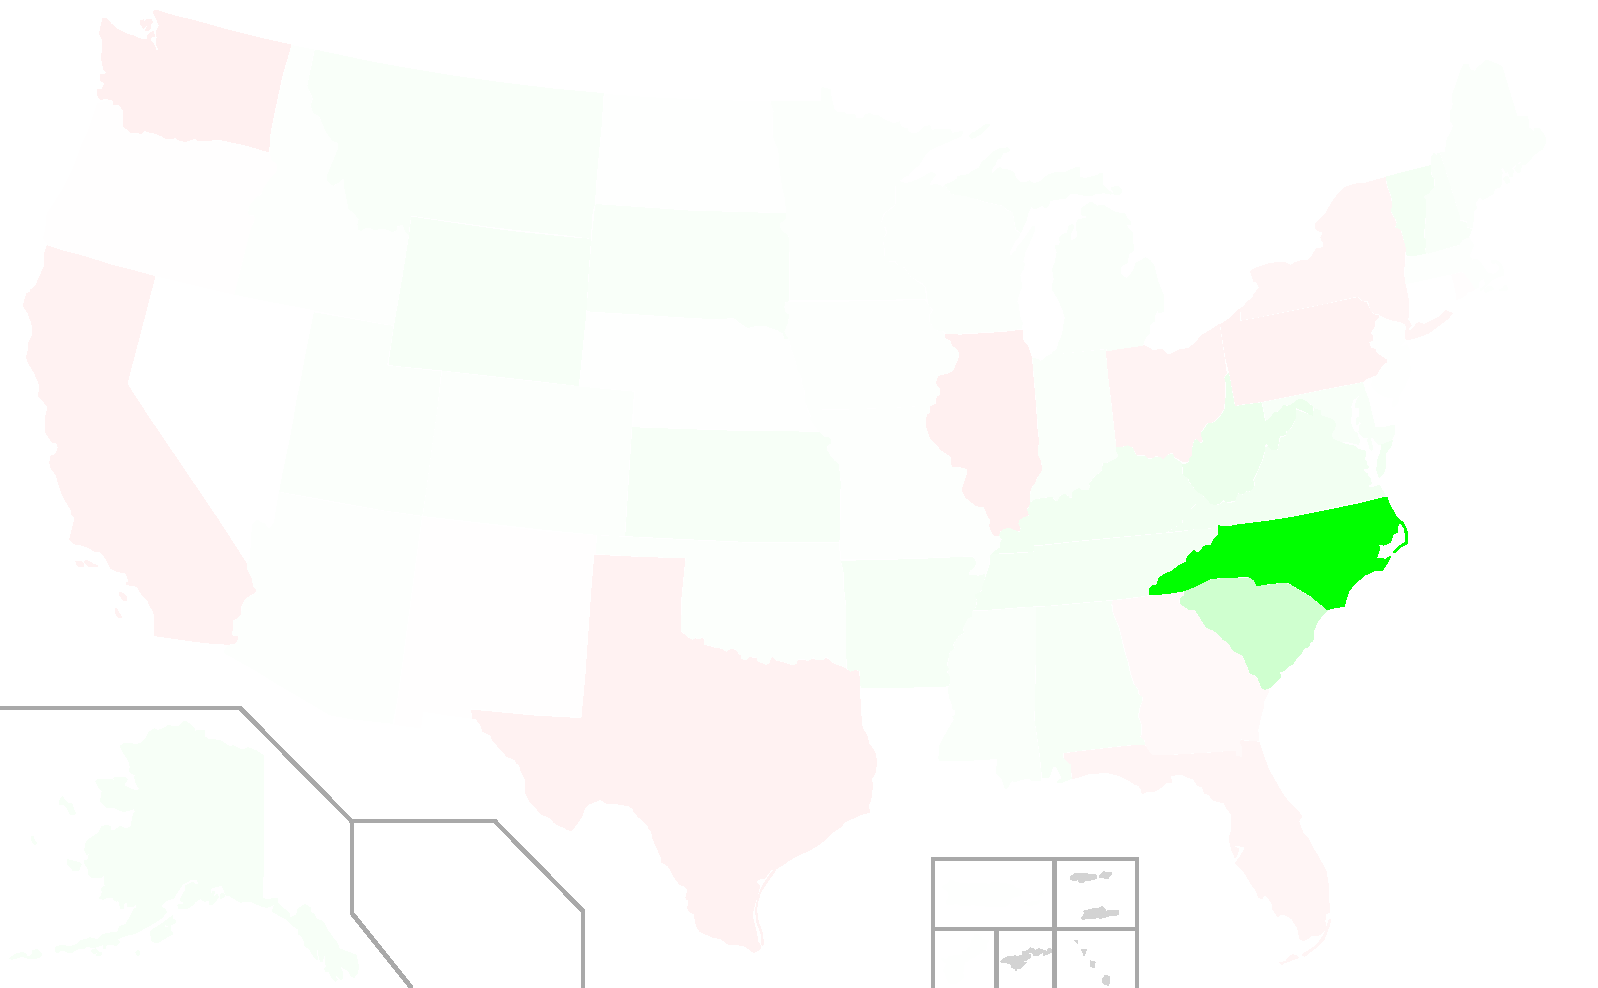
\includegraphics[width=53mm]{./images/nc.pdf}
\caption{Followers of North Carolina}
\label{fig:state-nc}
\end{minipage}
\end{figure*}
\end{center}

Our results are visualized for each attribute in figures throughout this paper.  These figures can be interpretted as follows: the groupings that are orderd by row are following the groupings that are ordered by column.  To read the bias for a particular relationship in these charts, find the desired row grouping and move right across the page.  Negative bias relationships are shaded red, and indicate that a row group has a bias against following a particular column group.  Positive bias relationships are shaded green, and indicate that a row group is biased in favor of following a particular column group.  The shade color increases with the strength of the bias.  Relationships that were not contained in our dataset are represented by gray-shaded empty squares.  For the sake of readability, the strength of shading is adjusted across different figures.  The strength of observed biases across different attributes is evaluated in \ref{sub:crossattribute}

Figure \ref{fig:follower_count}, a visualization of bias across follower count groupings, reveals a number of interesting facets of our Twitter subgraph.  One important feature is the values on the diagonal line moving from the top left to botthom right corner of the graph.  This line marks a group's affinity towards following itself, and will be referred to often in this section.  Here, we observe that our groupings are either neutral or subtly positively biased in favor of following their own group.  The strength of this bias increases with the number of followers.  The only exception to this trend is at the lowest follower count level, where our group is biased against following itself.  Across our results for the quantitative attributes it can be observed that users of extremely low degree exhibit unique behavior.

\begin{figure*}[t]
 \centering
 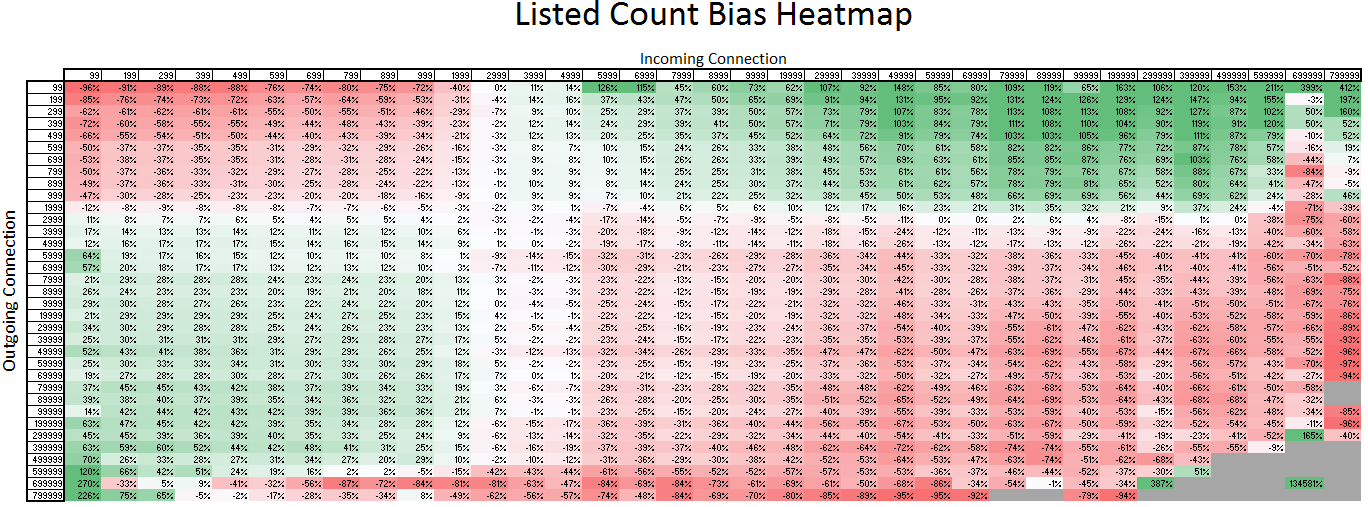
\includegraphics[bb=0 0 1026 380, scale=.3]{./images/Bates-Final/listedcount.png}
 % listedcount.png: 1368x507 pixel, 96dpi, 36.20x13.42 cm, bb=0 0 1026 380
 \label{fig:listed_count}
 \caption{A connectivity bias chart for number of lists a user appears on in logarithmically increasing groupings.}
\end{figure*}

\begin{figure*}[t]
 \centering
 \subfigure[A connectivity bias chart for users by their account creation date.  The upper bound for each range is displayed.  Groups are organized in reverse chronological order for consistency; rare users appear on the bottom and left. ]{
 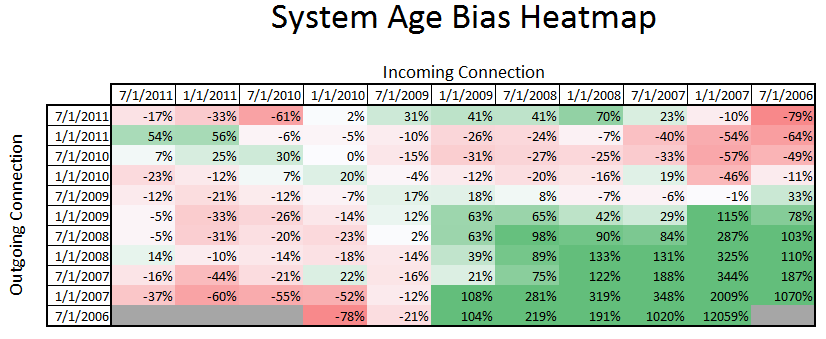
\includegraphics[bb=0 0 620 254, scale=.3]{./images/Bates-Final/sysage.png}
 % sysage.png: 826x339 pixel, 96dpi, 21.86x8.97 cm, bb=0 0 620 254
 \label{fig:sysage}
 }
 \subfigure[A connectivity bias chart for users by language setting.]{
 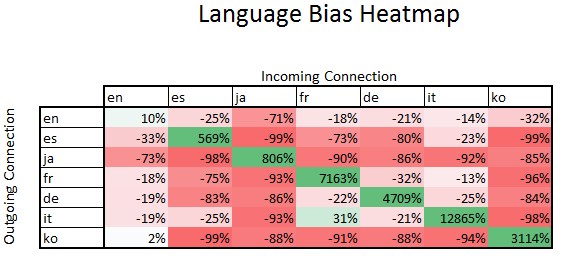
\includegraphics[bb=0 0 424 194, scale=.4]{./images/Bates-Final/lang.png}
 % lang.png: 565x259 pixel, 96dpi, 14.95x6.85 cm, bb=0 0 424 194
 \label{fig:lang}
 }
\end{figure*}

<<<<<<< HEAD
\begin{figure*}[t]
=======
Figure \ref{fig:protected} displays connectivity bias based on whether or not a user's messages are protected.  The only considerable bias displayed in this chart is that users with protected accounts are biased against following one another.  Figure \ref{fig:geoenabled} displays significant positive bias for all relationships featuring non-geoenabled user groupings as well as a negative bias for \textit{Geoenabled follows Geoenabled}.

Figures \ref{fig:state-ca}-\ref{fig:state-nc} show connectivity bias for the top 10 U.S. states, within the set of edges going to or coming from those states.  In general, states show a tendancy towards following themselves, and are followed by bordering states.  In the case of California, all states except the remaining top 9 are biased toward following California.  The mostly consistent bias against followers from the top 10 states is likely due to their being central to this analysis.

\begin{figure}[t]
 \centering
 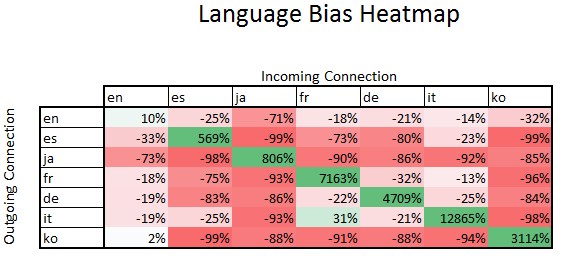
\includegraphics[bb=0 0 424 194, scale=.5]{./images/Bates-Final/lang.png}
 % lang.png: 565x259 pixel, 96dpi, 14.95x6.85 cm, bb=0 0 424 194
 \caption{A connectivity bias chart for users by language setting.}
 \label{fig:lang}
\end{figure}

\begin{figure}[t]
>>>>>>> 47f543aaa161944299cb39434309eb916ff3195c
 \centering
 \subfigure[A connectivity bias chart for whether or not the user's account is protected.]{
 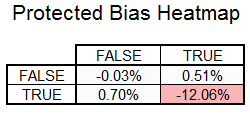
\includegraphics[bb=0 0 188 86, scale=.5]{./images/protected.png}
 % protected.png: 250x114 pixel, 96dpi, 6.62x3.02 cm, bb=0 0 188 86
 \label{fig:protected}
<<<<<<< HEAD
 }
\hspace{30 mm}
 \subfigure[A connectivity bias chart for whether or not the user's account is geo-enabled to include location information with each tweet.]{
=======
\end{figure}

\begin{figure}[t]
 \centering
>>>>>>> 47f543aaa161944299cb39434309eb916ff3195c
 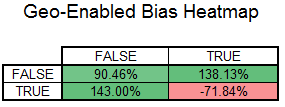
\includegraphics[bb=0 0 214 80, scale=.5]{./images/geoenabled.png}
 % geoenabled.png: 285x107 pixel, 96dpi, 7.54x2.83 cm, bb=0 0 214 80
 \label{fig:geoenabled}
 }
\end{figure*}

<<<<<<< HEAD
Moving away from the downward diagonal in either direction, it can be seen that groups become increasingly biased against following one another.  It looks as though this trend begins to dissipate once the degree of the incoming connection increases to above 50,000.  Unfortunately, this is obscured by the absence of a number of relationships that were not contained in our dataset.  The column for 199,999 represents only a single account in our subgraph, which is why the relationship transitions are so distinct.  This column is not being considered.

Figure \ref{fig:friend_count}, a visualization of bias for the friend count attribute, contains much of the same trends that are observed in Figure \ref{fig:follower_count}.  A subtle bias towards following users of a similar friend count is clearly visible here along the chart's diagonal.  This bias grows stronger once the grouping being follower reaches a degree of greater than 2000, at which point there is extremely strong bias in favor of following users from these groups.  Unlike with follower count, low degree users follow eachother at a frequency above that which would be expected in an unbiased network.

Figure \ref{fig:status_count} displays bias patterns for user groupings by status count.  Our intuition here was that users would be that likely to connect to user accounts with different degrees of status count.  This intuition is confirmed in the graph.  When considering status count, groupings are biased against following their own group until the very high degree groupings.  Low degree tweeters appear to be following high degree tweeters.  High degree tweeters are biased towards following two different degree ranges of users, those of either a very low or very high degree.
=======
\subsection{Comparing Bias Across Different Attributes}
\label{sub:crossattribute}
CROSS ATTRIBUTE YEAAAAHHHHH!!!

\noindent \begin{tabular}[t]{| p{1in} | p{1.75in} | p{1in} | p{1in} | p{1.25in} |}
\hline
\textbf{Bias Pattern} & \textbf{Attribute} & \textbf{Direction} & \textbf{Strength}  \\ \hline
Location & User-reported geographic location. & 3481 & 3481  \\ \hline
Protected & If true, only approved followers may see the user's tweets & 2 & 2  \\ \hline
Followers Count & Number of users who track this user's tweets & 2116 & 2116 \\ \hline
Friends Count & Number of users this user follows & 2116 & 2116 \\ \hline
Account age & Difference between account creation date and current date & 169 & 169  \\ \hline
\end{tabular}
>>>>>>> 47f543aaa161944299cb39434309eb916ff3195c

Figure \ref{fig:utc_offset} displays attribute relationships for users in different parts of the world by their offset from coordinated universal time.  While, UTC Offset generally refers to a longitudinal slice of the globe, certain offsets are used exclusively by certain countries or regions.  We observe that the strongest positive bias in this chart is at UTC Offset +5.5 following UTC Offset -8.  These two offsets correspond to user accounts in India and Sri Lanka following user accounts in Pacific Standard Time.  All groupings displayed varying degrees of bias against following user accounts at UTC Offset +9, which corresponds to the time zone in Japan and North and South Korea.  It should be noted that some of relationships displayed in this chart were extremely rare in our subgraph and may not be reliable.
 
Figure \ref{fig:listed_count} displays connectivity bias based on the number of Twitter lists tha a user appears on.  Lists are a way to organize and separate different message streams, and our intuition here was that there would be a bias towards following users that appear more frequently on lists.  As it turns out, this trend is only present when considering users of a low listed count degree.  Groupings of users that appear on over 100 lists display a consistent and considerable bias against following other high degree listed count users.

<<<<<<< HEAD
Figure \ref{fig:protected} displays connectivity bias based on whether or not a user's messages are protected.  The only considerable bias displayed in this chart is that users with protected accounts are biased against following one another.  Figure \ref{fig:geoenabled} displays significant positive bias for all relationships featuring non-geoenabled user groupings as well as a negative bias for \textit{Geoenabled follows Geoenabled}.

Figures \ref{fig:follower_count}, \ref{fig:friend_count} likely speak to two distinct purposes for which Twitter is used.  The bias for the protected and geoenabled attributes likely share a common bond.  The enabling of these options likely indicates that a user wishes to use Twitter amongst a small group of known friends.  High profile, influential public users will not generally have these options enabled.  Since our premise is that there is a bias in the Twitter network towards following influential users, it stands to reason that there is a negative bias in a relationship between two groupings that does not contain these rare users.

\subsection{Comparing Bias Across Different Attributes}
\label{sub:crossattribute}
While analyizing each attribute, we indentified several recurring bias patterns through which the attributes can be compared.  Each attribute can be described by its behavior across these bias patterns.  Across all attributes, we observed \textit{group follows itself} and \textit{group follows others} patterns.  There are additional patterns for attributes of continuous range -- \textit{low degree follows low degree}, \textit{high degree follows high degree}, \textit{low degree follows high degree}, and \textit{high degree follows low degree}.
=======
\subsection{Observations}
Conclude that across these attributes there are several identifiable patterns -- similar users follow eachother, dissimilar users follow eachother, low degree users follow high degree users, extreme low degree users deviate from general usage, extreme high degree users deviate from general usage.  Identify which attributes belong to which patterns.\\

Figures \ref{fig:follower_count}, \ref{fig:friend_count} and \ref{fig:status_count} likely speak to two distinct purposes for which Twitter is used.
>>>>>>> 47f543aaa161944299cb39434309eb916ff3195c

The bias for the protected and geoenabled attributes likely share a common bond.  The enabling of these options likely indicates that a user wishes to use Twitter amongst a small group of known friends.  High profile, influential public users will not generally have these options enabled.  Since our premise is that there is a bias in the Twitter network towards following influential users, it stands to reason that there is a negative bias in a relationship between two groupings that does not contain these rare users.
